\documentclass[a4paper,12pt]{article}

%\usepackage[italian]{babel}
\usepackage{graphicx}
\usepackage[absolute,overlay]{textpos}
\usepackage{anyfontsize}
\usepackage{etoolbox}
\usepackage{array}
\usepackage{longtable}
\usepackage{caption}
\usepackage{geometry}
\geometry
{ a4paper,
  total={170mm,250mm},
  left=20 mm,
  right=20mm,
  top=25mm ,
  bottom=20mm}
\def\doubleunderline#1{\underline{\underline{#1}}}

\makeatletter
\patchcmd{\@maketitle}{\vskip 2em}{\vspace*{-2cm}}{}{}
\makeatother

\pagenumbering{gobble}

%Code Colors&Features
\usepackage{listings}
\usepackage{xcolor}

\definecolor{codegreen}{rgb}{0,0.6,0}
\definecolor{codegray}{rgb}{0.5,0.5,0.5}
\definecolor{codepurple}{rgb}{0.58,0,0.82}
\definecolor{backcolour}{rgb}{0.95,0.95,0.92}

\lstdefinestyle{mystyle}{
    backgroundcolor=\color{backcolour},   
    commentstyle=\color{codegreen},
    keywordstyle=\color{magenta},
    numberstyle=\tiny\color{codegray},
    stringstyle=\color{codepurple},
    basicstyle=\ttfamily\footnotesize,
    breakatwhitespace=false,         
    breaklines=true,                 
    captionpos=b,                    
    keepspaces=true,                 
    numbers=left,                    
    numbersep=5pt,                  
    showspaces=false,                
    showstringspaces=false,
    showtabs=false,                  
    tabsize=2
}

\lstset{style=mystyle}


\usepackage{makeidx}
\makeindex


\begin{document}

\title { \large \textsc{Università degli Studi di Napoli Federico II \\
		 Scuola Politecnica e delle Scienze di Base} \\
\textsc{Dipartimento di Ingegneria Elettrica e Tecnologie dell’Informazione}}

\author{}
\date{}
\maketitle 
\thispagestyle{empty}

\vspace*{-2cm}
\begin{center}
	\begin{figure}[h]
	\centering
 	
\includegraphics[width=0.3\textwidth]{unina_logo.png}
	\end{figure}
	
	\Large \textsc{Corso di laurea in Informatica \\
		   Insegnamento di Basi di Dati I\\
		   Anno Accademico 2019-2020}
\end{center}

\vspace*{+1.5cm}
\begin{center}
\Huge \bf Progettazione e sviluppo di una base di dati relazionale di un software gestionale per recensioni turistiche
\end{center}


\vspace*{-2cm}
\vfill 
\begin{flushleft}
\textit{Autori: \hfill Docenti:}


\normalsize{\textsc{Davide Pio Faicchia \hfill Prof. Francesco Cutugno} 


\textsc{MATRICOLA : N86003018 \hfill Dott. Marco Grazioso}


\textit{da.faicchia@studenti.unina.it}}
\end{flushleft}


\begin{flushleft}
\normalsize{\textsc{Mauro Guida}


\textsc{MATRICOLA : N86002889}


\textit{maur.guida@studenti.unina.it}}
\end{flushleft}


\newpage\null\thispagestyle{empty}
\begin{center}
\vfil
\vfil
\textit{Questa pagina è stata lasciata intenzionalmente bianca. } 
\vfil
\vfil 
\end{center}
\newpage

\newpage\null\pagenumbering{arabic}\setcounter{page}{3}
\begin{flushleft}
\vspace{-1.5cm}
\begingroup
\fontsize{35pt}{12pt}\selectfont\bf{Indice}
\endgroup
\vspace*{+1cm}


\Large\textsc{\bf Capitolo 1}\\
\hspace{+1cm} \large Analisi del problema \hfill 5\\

\Large\textsc{\bf Capitolo 2}\\
\hspace{+1cm}\large Progettazione concettuale \hfill 6\\
\hspace{+2cm}\large 2.1 Dizionario delle classi \hfill 7\\
\hspace{+2cm}\large 2.2 Dizionario delle associazioni \hfill 9\\
\hspace{+2cm}\large 2.3 Dizionario dei vincoli \hfill 10\\

\Large\textsc{\bf Capitolo 3}\\
\hspace{+1cm}\large Progettazione logica \hfill 12\\
\hspace{+2cm}\large 3.1 Schema logico \hfill 12\\
\hspace{+3cm}\normalsize 3.1.1 Traduzione delle associazioni \hfill 13\\

\Large\textsc{\bf Capitolo 4}\\
\hspace{+1cm}\large Progettazione fisica \hfill 14\\
\hspace{+2cm}\large 4.1 Note sull'implementazione \hfill 14\\
\hspace{+2cm}\large 4.2 Definizione delle tabelle \hfill 15\\
\hspace{+3cm}\normalsize 4.2.1 Definizione della tabella UTENTE \hfill 15\\
\hspace{+3cm}\normalsize 4.2.2 Definizione della tabella MAPPA \hfill 15\\
\hspace{+3cm}\normalsize 4.2.3 Definizione della tabella BUSINESS \hfill 16\\
\hspace{+3cm}\normalsize 4.2.4 Definizione della tabella RECENSIONE \hfill 16\\
\hspace{+3cm}\normalsize 4.2.5 Definizione della tabella ASSOCIAZIONERAFFINAZIONE \hfill 17\\
\hspace{+3cm}\normalsize 4.2.6 Definizione della tabella IMMAGINEPROPRIETA \hfill 17\\
\hspace{+3cm}\normalsize 4.2.7 Definizione della tabella IMMAGINERECENSIONE \hfill 17\\
\hspace{+2cm}\large 4.3 Funzioni, procedure e Trigger \hfill 18\\
\hspace{+3cm}\normalsize 4.3.1 Integrità delle raffinazioni per tipologia 'Ristorante' \hfill 18\\
\hspace{+3cm}\normalsize 4.3.2 Integrità delle raffinazioni per tipologia 'Alloggio' \hfill 18\\
\hspace{+3cm}\normalsize 4.3.3 Integrità delle raffinazioni per tipologia 'Attrazione' \hfill 19\\
\hspace{+3cm}\normalsize 4.3.4 Generazione codice verifica per Utente \hfill 20\\
\hspace{+3cm}\normalsize 4.3.5 Effettua login \hfill 20\\
\hspace{+3cm}\normalsize 4.3.6 Effettua la registrazione \hfill 20\\
\hspace{+3cm}\normalsize 4.3.7 Imposta nuova passoword \hfill 21\\
\hspace{+3cm}\normalsize 4.3.8 Controlla documenti utente \hfill 21\\
\hspace{+3cm}\normalsize 4.3.9 Controlla codice verifica \hfill 21\\
\hspace{+3cm}\normalsize 4.3.10 Inserisci documenti utente \hfill 22\\
\hspace{+3cm}\normalsize 4.3.11 Inserisci business \hfill 22\\
\hspace{+3cm}\normalsize 4.3.12 Inserisci immagini a business\hfill 22\\
\hspace{+3cm}\normalsize 4.3.13 Recupera codice business\hfill 23\\
\hspace{+3cm}\normalsize 4.3.14 Inserisci raffinazioni\hfill 23\\
\hspace{+3cm}\normalsize 4.3.15 Funzione INSTR\hfill 24\\
\hspace{+3cm}\normalsize 4.3.17 Inserisci immagine recensione\hfill 24\\
\hspace{+3cm}\normalsize 4.3.16 Inserisci recensione\hfill 25\\
\hspace{+3cm}\normalsize 4.3.18 Ricerca locale\hfill 25\\
\hspace{+3cm}\normalsize 4.3.19 Aggiorna media stelle\hfill 26\\
\hspace{+3cm}\normalsize 4.3.20 Utente con recensione\hfill 26\\
\hspace{+2cm}\large 4.4 Chiamate SQL integrate nell'Applicativo \hfill 27\\
\hspace{+3cm}\normalsize 4.4.1 Recupera locali da ricerca\hfill 27\\
\hspace{+3cm}\normalsize 4.4.2 Recupera locali da tipo\hfill 27\\
\hspace{+3cm}\normalsize 4.4.3 Recupera business da codUtente\hfill 27\\

\end{flushleft}
\newpage

\newpage\null\pagenumbering{arabic}\setcounter{page}{5} 
\begin{flushleft}

\vspace*{+1cm}
\Large\textsc{\bf Capitolo 1}
\vspace*{+1cm}

\begingroup
\fontsize{35pt}{12pt}\selectfont\bf{Analisi del problema}
\endgroup
\vspace*{+1cm}
\end{flushleft}

\normalsize{
In questo primo capitolo verrà presentata una panoramica generale analizzato il problema al livello di astrazione più alto.
\vspace*{+0.2cm}
\\E' stata richiesta la progettazione di una base di dati relazionale per un software di recensioni turistiche, il focus del problema è stato, quindi, gestire un numero indefinito di utenti, permettendo loro l'inserimento in piattaforma di recensioni e nuove attività a scopo pubblicitario e valutativo delle stesse, su tutto il territorio nazionale (Italia).
\vspace*{+0.2cm}
\\Da come è possibile analizzare dal {\it class diagram} al Capitolo 2, il concetto cardine del software presentato è il concetto di {\bf Business }, al quale è permesso a uno o più utenti di associarvi una recensione, accompagnata, o meno, da immagini e descrizione.
\vspace*{+0.2cm}
\\Tale implementazione ha richiesto l'uso di 7 Tabelle e 2 Enumerazioni, come riportato graficamente al Capitolo 2 e descritto ampiamente al paragrafo 1 del medesimo capitolo. Lo sviluppo, in oltre, non ha richiesto la ristrutturazione del {\it class diagram} in quanto non presenti specializzazioni o associazioni molti a molti. La completa descrizione delle tabelle e le relative associazioni può essere osservata al Capitolo 3.
\vspace*{+0.2cm}
\\Ove possibile si è preferito evitare un'interazione diretta tra l'applicativo sviluppato ed il database. Per soddisfare tale scelta implementativa si è preferito dotare il database di funzioni specifiche (4.3), fornendo all'applicativo solo le informazioni strettamente necessarie alla corretta visualizzazione delle informazioni.
\vspace*{+0.2cm}
\\Onde evitare alterazioni {\it non} volontarie da parte del personale addetto alla manutenzione, con accesso diretto alla struttura dati, ogni vincolo è implementato direttamente nel database, così da impedire l'errato inserimento o modifica delle tabelle, limitando la possibilità di portare il sistema in uno stato instabile. Il \textit{dizionario dei vincoli} può essere consultato al Capitolo 2 (2.3), dove è riportata anche una descrizione degli stessi.
\vspace*{+0.2cm}
\\Da qui in avanti saranno usati in modo intercambiabile i termini \textit{Attività} e \textit{Business}.
}

\newpage 


\newpage\null\pagenumbering{arabic}\setcounter{page}{6}
\begin{flushleft}

\vspace*{+1cm}
\Large\textsc{\bf Capitolo 2}
\vspace*{+1cm}

\begingroup
\fontsize{30pt}{12pt}\selectfont\bf{Progettazione concettuale}
\endgroup
\vspace*{+1cm}
\end{flushleft}

\begin{center}
	\begin{figure}[h]
	\centering
 	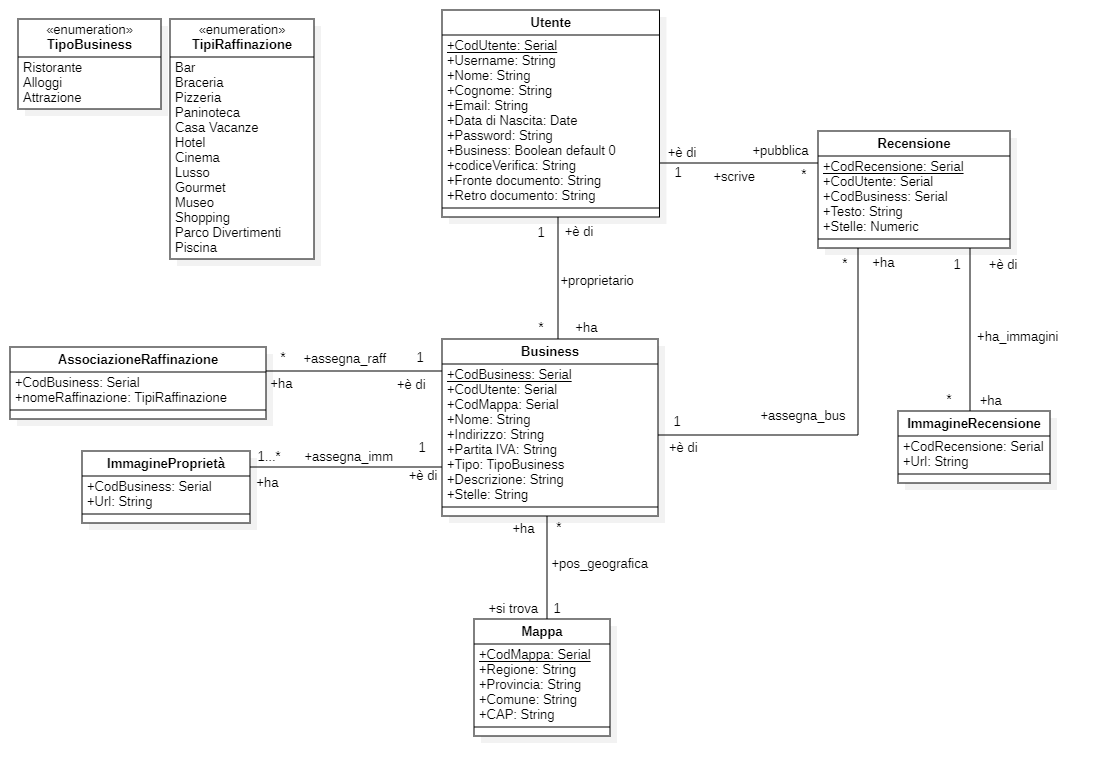
\includegraphics[width=0.8\textwidth]{classDiagram.png}
	\end{figure}

\end{center}

\normalsize{
{\small \it* Durante lo sviluppo del progetto non è stato necessario ristrutturare il  class diagram}.
\vspace*{+0.2cm}
\\Le associazioni tra tabelle avvengono tramite l'uso delle chiavi primarie: CodUtente, CodBusiness, CodRecensione e CodMappa. Come si evince dal nome, tali chiavi indicano univocamente: Utenti, Attività, Recensioni di un determinato utente ad un determinato Business e uno specifico luogo sulla mappa.
\vspace*{+0.2cm}
\\Affinché fosse possibile categorizzare un Business, si sono dovuti creare delle tabelle enumerazione per definire dei tipi specifici per le 3 Attività da gestire (Ristorante, Alloggio, Attrazione) e le relative specializzazioni (4.3.1).
\vspace*{+0.2cm}
\\Un'ampia descrizione delle Classi utilizzate e i relativi vincoli, può essere consultata nei paragrafi immediatamente successivi.
}

\newpage

\newpage\null\pagenumbering{arabic}\setcounter{page}{7}
\vspace{-2cm}
\begin{flushleft}
{\bf 2.1 Dizionario delle classi} 
\vspace{+1cm}
\begin{table}[htbp]
\begin{tabular}[c]{| m{3cm} | m{5cm} | m{7cm} |}
\hline
\bf Classe&\bf Descrizione&\bf Attributi\\
\hline
% 1 riga
{\bf Business}
&\small Descrittore di ciascuna attività presente nel portale
&\footnotesize
{\bf CodBusiness}({\it serial}): chiave primaria. Identifica univocamente ciascuna attività.

{\bf Nome}({\it varchar}): nome dell'attività.

{\bf Indirizzo}({\it varchar}): indirizzo dell'attività.

{\bf PartitaIVA}({\it varchar}): partitaIVA associata all'attività.

{\bf tipo}({\it tipoBusiness}): tipologia dell'attività.

{\bf Descrizione}({\it varchar}): descrizione attività.

{\bf Stelle}({\it numeric}): valutazione corrente.

{\bf Telefono}({\it varchar}): numero telefonico.

{\bf codUtente}({\it integer}): chiave esterna. proprietario dell'attività. chiave esterna.

{\bf codMappa}({\it integer}): chiave esterna. posizione dell'attività. 
\\
\hline

% 2 riga
{\bf Utente}
&\small Descrittore degli utenti 
&\footnotesize
{\bf CodUtente}({\it serial}): chiave primaria. Identifica univocamente ciascun utente.

{\bf Username}({\it varchar}): username utilizzato dall'utente durante la
registrazione.

{\bf Nome}({\it varchar}): nome dell'utente.

{\bf Cognome}({\it varchar}): cognome dell'utente.

{\bf Email}({\it varchar}): email dell'utente.

{\bf DataDiNascita}({\it date}): data nascita dell'utente.

{\bf Password}({\it varchar}): password dell'utente.

{\bf CodiceVerifica}({\it varchar}): codice di verifica
utilizzato dall'utente durante la registrazione.

{\bf FronteDocumento}({\it varchar}): immagine fronte documento inserita 
dall'utente per pubblicare una propria attività.

{\bf RetroDocumento}({\it varchar}): immagine retro documento inserita 
dall'utente per pubblicare una propria attività.
\\
\hline

% 3 riga
{\bf Recensione}
&\small Descrittore delle recensioni inserite dagli utenti 
&\footnotesize
{\bf CodRecensione}({\it serial}): chiave primaria. Identifica univocamente ciascuna recensione.

{\bf Nome}({\it varchar}): testo della recensione.

{\bf Stelle}({\it numeric}): valutazione locale inserita nella recensione.

{\bf codUtente}({\it integer}): chiave esterna. identifica l'utente che 
ha scritto la recensione. 

{\bf codBusiness}({\it integer}): chiave esterna. identifica l'attività a
cui è associata la recensione.
\\
\hline

\multicolumn{3}{c}{\footnotesize{\normalsize *Tabella 1 :\it continua a pagina successiva}}
\end{tabular}

\end{table}
\end{flushleft}

\newpage


\newpage\null\pagenumbering{arabic}\setcounter{page}{8}
\vspace{-2cm}
\begin{table}[htbp]
\caption*{Tabella 1: {\it continua dalla pagina precedente.}}
\begin{tabular}[c]{| m{3cm} | m{5cm} | m{7cm} |}
\hline
\bf Classe&\bf Descrizione&\bf Attributi\\
\hline
% 4 riga
{\bf Mappa}
&\small Descrittore della posizione geografica di ciascuna attività
&\footnotesize

{\bf CodMappa}({\it serial}): chiave primaria. Identifica univocamente ciascuna posizione geografica.

{\bf Stato}({\it varchar}): Attributo di locazione.

{\bf CAP}({\it varchar}): Attributo di locazione.

{\bf Comune}({\it varchar}): Attributo di locazione.

{\bf Provincia}({\it varchar}): Attributo di locazione.

{\bf Regione}({\it varchar}): Attributo di locazione.

{\bf SiglaProvincia}({\it varchar}): Attributo di locazione.
\\
\hline

% 5 riga
{\bf Immagine
Proprietà}
&\small Descrittore delle immagini inserite dal proprietario associate ad una propria
attività.
&\footnotesize
{\bf URL}({\it varchar}): URL dell'immagine.

{\bf codBusiness}({\it integer}): chiave esterna. Identifica l'attività a
cui è associata l'immagine.
\\
\hline

% 6 riga
{\bf Associazione
Raffinazione}
&\small Descrittore delle raffinazioni di tipologia associate a ciascuna attività.
&\footnotesize
{\bf raffinazione}({\it tipoRaffinazione}): Raffinazione di una tipologia di attività.

{\bf codBusiness}({\it integer}): chiave esterna. Identifica l'attività a
cui è associata la raffinazione specificata.
\\
\hline

% 7 riga
{\bf Immagine
Recensione}
&\small Descrittore delle immagini associate a ciascuna recensione.
&\footnotesize
{\bf URL}({\it varchar}): URL dell'immagine.

{\bf codRecensione}({\it integer}): chiave esterna. Identifica la recensione a 
cui è stata associata l'immagine.
\\
\hline
\multicolumn{3}{c}{\footnotesize{\normalsize Tabella 1 - Dizionario delle classi}}
\end{tabular}
\end{table}
\newpage


\newpage\null\pagenumbering{arabic}\setcounter{page}{9}
\vspace{-2cm}
\begin{flushleft}
{\bf 2.2 Dizionario delle associazioni} 
\vspace{+1cm}
\begin{table}[htbp]
\begin{tabular}[c]{| m{3cm} | m{5cm} | m{7cm} |}
\hline
\bf Nome&\bf Descrizione&\bf Classi coinvolte\\
\hline
{\bf assegna\_raff}
&\small esprime l'assegnazione di una raffinazione di tipologia
a un business.
&\footnotesize
{\bf Business[1]} ruolo {\bf è di}: indica l'attività a cui viene 
assegnata la raffinazine.

{\bf AssociazioneRaffinazione[0..*]} ruolo {\bf ha}: esprime la possibilità di associare a un'attivita delle raffinazioni
\\
\hline

{\bf pos\_geografica}
&\small esprime l'assegnazione di un'attività alla propria posizione
geografica (in termini di CAP, Regione, Comune,...)
&\footnotesize
{\bf Business[0..*]} ruolo {\bf ha}: esprime la condizione per la quale
una stessa posizione geografica può essere assegnata a più attività.

{\bf Mappa[1]} ruolo {\bf si trova}: indica la posizione geografica
associata al business.
\\
\hline

{\bf assegna\_imm}
&\small esprime l'assegnazione di una certa immagine a una attività.
&\footnotesize
{\bf Business[1]} ruolo {\bf è di}: esprime il business al quale è
associata la coppia ({\it url,codBusiness}).

{\bf ImmagineProprietà[1..*]} ruolo {\bf ha}: esprime l'immagine associata
al business in termini di coppia ({\it url,codBusiness}).
\\
\hline

{\bf proprietario}
&\small esprime l'assegnazione di una certa attività al suo proprietario
&\footnotesize
{\bf Business[0..*]} ruolo {\bf ha}: esprime la condizione per la quale
un certo utente può o non avere un'attività.

{\bf Utente[1]} ruolo {\bf è di}: definisce il proprietario dell'attività.
\\
\hline

{\bf scrive}
&\small esprime l'assegnazione di una recensione all'utente che l'ha 
scritta.
&\footnotesize
{\bf Recensione[0..*]} ruolo {\bf pubblica}: esprime la possibilità per un
utente di scrivere o meno delle recensioni.

{\bf Utente[1]} ruolo {\bf è di}: definisce l'utente che ha scritto la
recensione.
\\
\hline

{\bf assegna\_bus}
&\small esprime l'assegnazione di una certa recensione ad un'attività.
&\footnotesize
{\bf Business[1]} ruolo {\bf è di}: definisce il business a cui è
associata la recensione

{\bf Recensione[0..*]} ruolo {\bf ha}: definisce la possibilità di associare o meno una recensione ad un'attività.
\\
\hline

{\bf ha\_immagini}
&\small esprime l'assegnazione di una certa immagine ad una recensione.
&\footnotesize
{\bf ImmagineRecensione[0..*]} ruolo {\bf ha}: indica la possibilità per 
una recensione di avere o meno delle immagini associate.

{\bf Recensione[1]} ruolo {\bf è di}: definisce la recensione ha cui viene
associata una certa immagine.
\\
\hline
\multicolumn{3}{c}{\footnotesize{\normalsize Tabella 2 - Dizionario delle associazioni}}
\end{tabular}
\end{table}
\end{flushleft}
\newpage


\newpage\null\pagenumbering{arabic}\setcounter{page}{10}
\vspace{-2cm}
\begin{flushleft}
{\bf 2.3 Dizionario dei vincoli} 
\vspace{+1cm}
\begin{table}[htbp]
\begin{tabular}[c]{| m{6cm} | m{10cm} |}
\hline
\bf Nome Vincolo&\bf Descrizione\\
\hline

{\bf legit emails}
&\small Le emails inserite dagli utente devono avere un formato leggittimo, ergo devono contenere almeno un carattere prima della @ , almeno un carattere tra essa e il punto e almeno due caratteri nella parte
finale.
vedi: {\it 4.2.1 Definizione della tabella UTENTE}.
\\
\hline

{\bf LunghezzaPassword}
&\small Le password inserite dagli utenti devono avere lunghezza maggiore o uguale di 6.
vedi: {\it 4.2.1 Definizione della tabella UTENTE}.
\\
\hline

{\bf RecensioneUnicaUtenteLuogo}
&\small Un utente può pubblicare al più una recensione per attività.
vedi: {\it 4.2.4 Definizione della tabella RECENSIONE}.
\\
\hline

{\bf RaffinazioneUnica}
&\small Non è possibile associare più di una volta una stessa raffinazione a una attività.
vedi: {\it 4.2.5 Definizione della tabella ASSOCIAZIONERAFFINAZIONE}.
\\
\hline

{\bf NumeroDiTelefonoNonValido}
&\small I numeri di telefono dei business devono avere un formato leggittimo. Devono contentere 10 cifre.
vedi: {\it 4.2.3 Definizione della tabella BUSINESS}.
\\
\hline

{\bf NumeroDiTelefono
TroppoCorto}
&\small I numeri di telefono dei business devono avere un formato leggittimo. Devono contentere solo cifre numeriche.
vedi: {\it 4.2.3 Definizione della tabella BUSINESS}.
\\
\hline

{\bf lunghezzaPartitaIVA}
&\small La partitaIVA deve avere esattamente 10 caratteri.
vedi: {\it 4.2.3 Definizione della tabella BUSINESS}.
\\
\hline

{\bf DataDiNascita
NonValida}
&\small Non è possibile che l'utente sia nato nell'istante presente o nel futuro.
vedi: {\it 4.2.1 Definizione della tabella UTENTE}.
\\
\hline

{\bf noImmagineProprieta}
&\small Non è possibile associare più volte una stessa immagine a un business.
vedi: {\it 4.2.6 Definizione della tabella IMMAGINEPROPRIETA}.
\\
\hline

{\bf checkRaffinazioneRistoranti}
&\small vedi: {\it 4.3.1 Integrità delle raffinazioni per tipologia 'Ristorante'}.
\\
\hline

{\bf checkRaffinazioneAlloggio}
&\small vedi: {\it 4.3.2 Integrità delle raffinazioni per tipologia 'Alloggio'}.
\\
\hline

{\bf checkRaffinazioneAttrazioni}
&\small vedi: {\it 4.3.3 Integrità delle raffinazioni per tipologia 'Attrazione'}.
\\
\hline

{\bf legit Stelle Business}
&\small Un business può avere (Stelle IS NULL) o meno una valutazione((Stelle BETWEEN 1 AND 5).
vedi: {\it 4.2.3 Definizione della tabella BUSINESS}.
\\
\hline

\multicolumn{2}{c}{\footnotesize{\normalsize *Tabella 3 - {\it continua a pagina successiva}}}
\end{tabular}
\end{table}
\end{flushleft}
\newpage

\newpage\null\pagenumbering{arabic}\setcounter{page}{11}
\vspace{-2cm}
\begin{flushleft}
\begin{table}[htbp]
\caption*{Tabella 3: {\it continua dalla pagina precedente.}}
\begin{tabular}[c]{| m{6cm} | m{10cm} |}
\hline
\bf Nome Vincolo&\bf Descrizione\\
\hline
{\bf legit Stelle Recensione}
&\small Una recensione {\it deve} avere una valutazione((Stelle BETWEEN 1 AND 5).
vedi: {\it 4.2.4 Definizione della tabella RECENSIONE}.
\\
\hline

{\bf unique Username}
&\small Non è possibile che più utenti abbiano lo stesso Username.
vedi: {\it 4.2.1 Definizione della tabella UTENTE}.
\\
\hline

{\bf unique PartitaIVA}
&\small Non è possibile che più business abbiano lo stesso Username.
vedi: {\it 4.2.3 Definizione della tabella BUSINESS}.
\\
\hline

{\bf domain tipoRaffinazione}
&\small Vincolo di dominio attributo \verb|tipo| nella tabella \verb|BUSINESS|.
vedi: {\it 4.2.3 Definizione della tabella BUSINESS}.
\\
\hline

{\bf domain tipoRaffinazione}
&\small Vincolo di dominio attributo \verb|raffinazione| nella tabella \verb|ASSOCIAZIONERAFFINAZIONE|.
vedi: {\it 4.2.3 Definizione della tabella ASSOCIAZIONERAFFINAZIONE}.
\\
\hline

{\bf domain tipoBusiness}
&\small Vincolo di dominio attributo \verb|tipo| nella tabella \verb|BUSINESS|.
vedi: {\it 4.2.3 Definizione della tabella BUSINESS}.
\\
\hline
\multicolumn{2}{c}{\footnotesize{\normalsize Tabella 3 - Dizionario dei vincoli}}
\end{tabular}
\end{table}
\end{flushleft}
\newpage

\newpage\null\pagenumbering{arabic}\setcounter{page}{12}
\begin{flushleft}
\vspace*{+1cm}
\Large\textsc{\bf Capitolo 3}
\vspace*{+1cm}

\begingroup
\fontsize{30pt}{12pt}\selectfont\bf{Progettazione logica}
\endgroup
\vspace*{+1cm}

\normalsize{
In questo capitolo saranno presentati gli schemi logico e relazionali.
}

\vspace*{+1cm}
{\bf 3.1 Schema logico}
\vspace*{+0.5cm}

\begin{table}[htbp]
\begin{tabular}[c]{ p{3.5cm}  p{11.5cm} }
\setlength{\extrarowheight}{20pt}
{\bf UTENTE}
&({\bf \underline{codUtente}}, Username, Nome, Cognome, Email, Password, DataDiNascita, 
codiceVerifica, FronteDocumento, Retro Documento)
\\
\\
{\bf BUSINESS}
&({\bf \underline{codBusiness}}, Nome, Indirizzo, PartitaIVA, tipo, Descrizione, Stelle, Telefono,
\doubleunderline{codUtente}, \doubleunderline{codMappa})
\\
\\
{\bf MAPPA}
&({\bf \underline{codMappa}}, Stato, CAP, Regione, Comune, Provincia, SiglaProvincia)
\\
\\
{\bf RECENSIONE}
&({\bf \underline{codRecensione}}, Testo, Stelle, \doubleunderline{codUtente}, \doubleunderline{codBusiness})
\\
\\
{\bf IMMAGINE
PROPRIETA}
&(URL, \doubleunderline{codBusiness})
\\
\\
{\bf ASSOCIAZIONE
RAFFINAZIONE}
&(raffinazione, \doubleunderline{codBusiness})
\\
\\
{\bf IMMAGINE
RECENSIONE}
&(URL, \doubleunderline{codRecensione})
\\
\\
\multicolumn{2}{c}{\footnotesize{\normalsize Tabella 4 - Schema logico}}
\end{tabular}
\end{table}
\end{flushleft}
\newpage

\newpage\null\pagenumbering{arabic}\setcounter{page}{13}
\vspace{-2cm}
\begin{flushleft}
{\bf 3.1.1 Traduzione delle associazioni} 
\vspace{+1cm}

\begin{table}[htbp]
\begin{tabular}[c]{ p{3.5cm}  p{11.5cm} }
\hline
\bf Associazione&\bf Implementazione\\
\hline\\
{\bf assegna\_raff}
&\small Chiave esterna in ASSOCIAZIONERAFFINAZIONE $\rightarrow$ BUSINESS
\\
\\
{\bf pos\_geografica}
&\small Chiave esterna in BUSINESS $\rightarrow$ MAPPA
\\
\\
{\bf assegna\_imm}
&\small Chiave esterna in IMMAGINEPROPRIETA $\rightarrow$ BUSINESS
\\
\\
{\bf propretario}
&\small Chiave esterna in BUSINESS $\rightarrow$ UTENTE
\\
\\
{\bf scrive}
&\small Chiave esterna in RECENSIONE $\rightarrow$ UTENTE
\\
\\
{\bf assegna\_bus}
&\small Chiave esterna in RECENSIONE $\rightarrow$ BUSINESS
\\
\\
{\bf ha\_immagini}
&\small Chiave esterna in IMMAGINERECENSIONE $\rightarrow$ RECENSIONE
\\\\
\hline
\multicolumn{2}{c}{\footnotesize{\normalsize Tabella 5 - Traduzione
delle associazioni}}
\end{tabular}
\end{table}
\end{flushleft}
\newpage

\newpage\null\pagenumbering{arabic}\setcounter{page}{14}
\begin{flushleft}
\vspace*{+1cm}
\Large\textsc{\bf Capitolo 4}
\vspace*{+1cm}

\begingroup
\fontsize{30pt}{12pt}\selectfont\bf{Progettazione fisica}
\endgroup

\vspace*{+1cm}
\normalsize{
La base di dati verrà implementata sul DBMS \verb|PostgreSQL 11.7|
}
\end{flushleft}

{\flushleft \bf 4.1 Note sull'implementazione}
\\
\normalsize{
Al fine di agevolare lo sviluppo delle funzioni necessarie, ove possibile, saranno utilizzate funzioni e procedure caratteristiche dello standard del DBMS in questione. Tuttavia, alcune funzionalità come \verb|INSTR| appartenente ad \verb|ORACLE|, non disponibile su \verb|PostgreSQL|, saranno implementate manualmente come funzioni del seguente Database, discorso equivalente per l'implementazione di \verb|ASSERTION|, anch'essa rimpiazzata da una specifica procedure poiché non disponibili.
\vspace*{+0.2cm}
\\Nel seguente capitolo saranno mostrate le funzionalità implementate lato Database, quali: Vincoli su Tabelle, Procedure, Funzioni e Trigger, oltre ad evidenziare come ogni Tabella sia stata definita.
\vspace*{+0.2cm}
\\Nel paragrafo 4 saranno approfondite le funzioni implementate direttamente dell'applicativo e pertanto non presenti nel Database, tuttavia questa pratica, ove possibile, sia stata scongiurata per semplificare future manutenzioni ed implementazioni, rendendo possibile effettuare aggiornamenti esclusivamente lato Database senza rendere obsolete vecchie release degli applicativi.
\vspace*{+0.2cm}
\\L'obbiettivo principale è rendere ogni richiesta dell'utente una chiamata ad una funzione presente nella Base di Dati, limitando possibili manomissioni e garantendo una maggiore stabilità del sistema, oltre ad un supporto a lungo termine degli applicativi.
}

\newpage

\newpage\null\pagenumbering{arabic}\setcounter{page}{15}
\vspace{-2cm}
{\flushleft \bf 4.2 Definizione delle tabelle} 
\\
Seguono le definizioni delle tabelle utilizzate nella base di dati, con le relative descrizioni dei vincoli adottati, per gli attributi, di ognuna di esse.\\
\begin{center}
{\small \it * Alcune parole risulteranno essere grammaticalmente errate data l'incompatibilità dei caratteri speciali col DBMS.}
\end{center}
\vspace*{+1cm}

{\flushleft \bf 4.2.1  Definizione della tabella UTENTE}
\begin{lstlisting}[language=SQL]
/**
*	  TABELLA: UTENTE
*   Crea la tabella e implementa i vincoli piu semplici
*/
CREATE TABLE Utente(
  codUtente SERIAL PRIMARY KEY,
  Username VARCHAR(50) NOT NULL UNIQUE,
  Nome VARCHAR(50) NOT NULL,
  Cognome VARCHAR(50) NOT NULL,
  Email VARCHAR(100) NOT NULL UNIQUE CHECK(Email LIKE '_%@%.__%'),
  DataDiNascita date NOT NULL,
  Password VARCHAR(100) NOT NULL,
  codiceVerifica VARCHAR(10) DEFAULT NULL,
  FronteDocumento VARCHAR(1000) DEFAULT NULL,
  RetroDocumento VARCHAR(1000) DEFAULT NULL
);

-- Vincolo di lunghezza della password
ALTER TABLE Utente
	ADD CONSTRAINT LunghezzaPassword CHECK(length(Password)>=6);
  
-- Vincolo di integrita della DataDiNascita inserita dall'utente  
ALTER TABLE Utente
	ADD CONSTRAINT DataDiNascitaNonValida 
		CHECK(NOT(DataDiNascita >= date('now')));
\end{lstlisting}

\vspace*{+1cm}

{\flushleft \bf 4.2.2  Definizione della tabella MAPPA}
\begin{lstlisting}[language=SQL]
/**
*	  TABELLA: MAPPA
*   Crea la tabella e implementa i vincoli piu semplici
*/
CREATE TABLE Mappa(
    codMappa SERIAL PRIMARY KEY
    Stato VARCHAR(5),
    CAP VARCHAR(7),
    Comune VARCHAR(100),
    Regione VARCHAR(100),
    Provincia VARCHAR(100),
    SiglaProvincia VARCHAR(5),
);
\end{lstlisting}
\newpage

\newpage\null\pagenumbering{arabic}\setcounter{page}{16}
\vspace{-2cm}
{\flushleft \bf 4.2.3  Definizione della tabella BUSINESS}
\begin{lstlisting}[language=SQL]
/**
*	  TABELLA: BUSINESS
*   Crea la tabella e implementa i vincoli piu semplici
*/

-- Vincolo di dominio per l'attributo 'tipo'
CREATE TYPE tipoBusiness AS ENUM ('Attrazione', 'Alloggio', 'Ristorante');

CREATE TABLE Business(
  codBusiness SERIAL PRIMARY KEY,
  Nome VARCHAR(50) NOT NULL,
  Indirizzo VARCHAR(100) NOT NULL,
  PartitaIVA VARCHAR(100) NOT NULL UNIQUE,
  tipo tipoBusiness NOT NULL,
  Descrizione VARCHAR(2000) NOT NULL,
  Stelle NUMERIC DEFAULT NULL CHECK((Stelle BETWEEN 1 AND 5) 
  									 									OR Stelle IS NULL),
  Telefono VARCHAR(10) NOT NULL,
  codUtente INTEGER REFERENCES Utente(codUtente) ON DELETE CASCADE,
  codMappa INTEGER REFERENCES Mappa(codMappa)
);

-- Vincolo di correttezza del numero telefonico (deve contenere solo cifre)
ALTER TABLE Business
  ADD CONSTRAINT NumeroDiTelefonoNonValido CHECK(Telefono ~ '^[0-9 ]*$');

-- Vincolo di correttezza del numero telefonico (deve contenere esattamente 10 cifre)
ALTER TABLE Business
  ADD CONSTRAINT NumeroDiTelefonoTroppoCorto CHECK(LENGTH(Telefono) = 10);

-- Vincolo di correttezza sulla lunghezza della partitaIVA inserita
ALTER TABLE Business
  ADD CONSTRAINT lunghezzaPartitaIVA CHECK(LENGTH(PartitaIVA) = 11);
\end{lstlisting}

\vspace*{+1cm}

{\flushleft \bf 4.2.4  Definizione della tabella RECENSIONE}
\begin{lstlisting}[language=SQL]
/**
*	  TABELLA: RECENSIONE
*   Crea la tabella e implementa i vincoli piu semplici
*/
CREATE TABLE Recensione(
  CodRecensione SERIAL PRIMARY KEY,
  Testo VARCHAR(2000) NOT NULL,
  Stelle NUMERIC NOT NULL CHECK(Stelle BETWEEN 1 AND 5),
  CodBusiness INTEGER REFERENCES Business(codBusiness) ON DELETE CASCADE,
  CodUtente INTEGER REFERENCES Utente(codUtente) ON DELETE CASCADE
);

-- Non sara possibile per un utente recensire piu volte lo stesso business
ALTER TABLE Recensione
  ADD CONSTRAINT RecensioneUnicaUtenteLuogo UNIQUE(codBusiness, codUtente);
\end{lstlisting}
\newpage

\newpage\null\pagenumbering{arabic}\setcounter{page}{17}
\vspace{-2cm}
{\flushleft \bf 4.2.5  Definizione della tabella ASSOCIAZIONERAFFINAZIONE}
\begin{lstlisting}[language=SQL]
/**
*	  TABELLA: ASSOCIAZIONERAFFINAZIONE
*   Crea la tabella e implementa i vincoli piu semplici
*/

-- Vincolo di dominio per l'attributo 'raffinazione'
CREATE TYPE tipoRaffinazione AS 
ENUM ('Pizzeria', 'Braceria', 'FastFood',
'Paninoteca', 'Osteria', 'TavolaCalda',
'Taverna', 'Trattoria', 'Pesce',
'Cinema', 'Shopping','Monumento',
'Museo', 'ParcoGiochi', 'Piscina',
'Lounge', 'Hotel', 'Bed&Breakfast',
'Ostello', 'CasaVacanze' ,'Residence');

CREATE TABLE AssociazioneRaffinazione(
  codBusiness INTEGER REFERENCES Business(codBusiness) ON DELETE CASCADE,
  raffinazione tipoRaffinazione
);

-- Non sara possibile associare piu di una volta una stessa raffinazione a un business
ALTER TABLE AssociazioneRaffinazione
	ADD CONSTRAINT RaffinazioneUnica UNIQUE(codBusiness,raffinazione);
);
\end{lstlisting}

\vspace*{+1cm}

{\flushleft \bf 4.2.6  Definizione della tabella IMMAGINEPROPRIETA}
\begin{lstlisting}[language=SQL]
/**
*	  TABELLA: IMMAGINEPROPRIETA
*   Crea la tabella e implementa i vincoli piu semplici
*/
CREATE TABLE ImmagineProprieta(
  Url VARCHAR(1000),
  codBusiness INTEGER REFERENCES Business(codBusiness) ON DELETE CASCADE
);

-- Non sara possibile associare piu di una volta una stessa immagine a un business
ALTER TABLE ImmagineProprieta
  ADD CONSTRAINT noImmagineProprieta UNIQUE(Url,CodBusiness);
\end{lstlisting}

\vspace*{+1cm}

{\flushleft \bf 4.2.7  Definizione della tabella IMMAGINERECENSIONE}
\begin{lstlisting}[language=SQL]
/**
*	  TABELLA: IMMAGINERECENSIONE
*   Crea la tabella e implementa i vincoli piu semplici
*/
CREATE TABLE ImmagineRecensione(
  Url VARCHAR(1000) NOT NULL,
  codRecensione INTEGER REFERENCES Recensione(CodRecensione) ON DELETE CASCADE
);
\end{lstlisting}
\newpage

\newpage\null\pagenumbering{arabic}\setcounter{page}{18}
\vspace{-2cm}
{\flushleft \bf 4.3 Funzioni, procedure e Trigger}
\\In questo paragrafo verrà fornita una descrizione accurata dei metodi di automazione adottati, quali trigger e delle funzioni e procedure richiamate dall'applicativo con lo scopo di ricavare le informazioni necessarie al suo funzionamento.
\vspace*{+1cm}
\newline
{\bf 4.3.1  Integrità delle raffinazioni per tipologia 'Ristorante'}\\
\normalsize{Se l'utente seleziona come tipologia \verb|'Ristorante'|, allora le raffinazioni
devono essere necessariamente pescate tra le seguenti : \\
\verb|('Pizzeria', 'Braceria', 'FastFood', 'Paninoteca', 'Osteria', 'Tavola',|\\
\verb|'Taverna','Trattoria', 'Pesce')|}
\begin{lstlisting}[language=SQL]
CREATE FUNCTION checkRaffinazioneRistoranti() RETURNS TRIGGER AS
$BODY$
DECLARE
	raff AssociazioneRaffinazione.raffinazione%TYPE;
BEGIN
	FOR raff IN SELECT raffinazione FROM AssociazioneRaffinazione WHERE codBusiness = NEW.codBusiness
	LOOP
		IF raff.raffinazione NOT IN 
			('Pizzeria', 'Braceria', 'FastFood',
			 'Paninoteca', 'Osteria', 'Tavola Calda',
			 'Taverna','Trattoria', 'Pesce') THEN
			RAISE EXCEPTION 'Errore: Raffinazione non consentita';
		END IF;
	END LOOP;
END;
$BODY$
LANGUAGE PLPGSQL;


CREATE TRIGGER checkRaffinazioneRistoranti
BEFORE INSERT ON Business
FOR EACH ROW
WHEN (NEW.tipo = 'Ristorante')
EXECUTE PROCEDURE checkRaffinazioneRistoranti();
\end{lstlisting}
\vspace*{+1cm}

{\flushleft \bf 4.3.2  Integrità delle raffinazioni per tipologia 'Alloggio'}\\
\normalsize{Se l'utente seleziona come tipologia \verb|'Alloggio'|, allora le raffinazioni
devono essere necessariamente pescate tra le seguenti : \\
\verb|('Hotel', 'Bed&Breakfast', 'Ostello', 'CasaVacanze' ,'Residence')|}
\begin{lstlisting}[language=SQL]
CREATE FUNCTION checkRaffinazioneAlloggio() RETURNS TRIGGER AS
$BODY$
DECLARE
	raff AssociazioneRaffinazione.raffinazione%TYPE;
BEGIN
	FOR raff IN SELECT raffinazione FROM AssociazioneRaffinazione WHERE codBusiness = NEW.codBusiness
	LOOP
		IF raff.raffinazione NOT IN 
			('Hotel', 'Bed&Breakfast', 'Ostello', 'CasaVacanze' ,'Residence') THEN
			RAISE EXCEPTION 'Errore: Raffinazione non consentita';
		END IF;
	END LOOP;
END;
$BODY$
LANGUAGE PLPGSQL;


CREATE TRIGGER checkRaffinazioneAlloggio
BEFORE INSERT ON Business
FOR EACH ROW
WHEN (NEW.tipo = 'Alloggio')
EXECUTE PROCEDURE checkRaffinazioneAlloggio();
\end{lstlisting}
\vspace*{+1cm}

{\flushleft \bf 4.3.3 Integrità delle raffinazioni per tipologia 'Attrazione'}\\
\normalsize{Se l'utente seleziona come tipologia \verb|'Attrazione'|, allora le raffinazioni
devono essere necessariamente pescate tra le seguenti : \\
\verb|('Cinema', 'Shopping','Monumento', 'Museo', 'Parco Giochi', 'Piscina',|\\
\verb|'Bar/Lounge')|}
\begin{lstlisting}[language=SQL]
CREATE FUNCTION checkRaffinazioneAttrazioni() RETURNS TRIGGER AS
$BODY$
DECLARE
	raff AssociazioneRaffinazione.raffinazione%TYPE;
BEGIN
	FOR raff IN SELECT raffinazione 
			     FROM AssociazioneRaffinazione 
			     WHERE codBusiness = NEW.codBusiness LOOP
		IF raff.raffinazione NOT IN 
		   ('Cinema', 'Shopping','Monumento', 'Museo', 
		    'Parco Giochi', 'Piscina', 'Bar/Lounge') THEN
			RAISE EXCEPTION 'Errore: Raffinazione non consentita';
		END IF;
	END LOOP;
END;
$BODY$
LANGUAGE PLPGSQL;


CREATE TRIGGER checkRaffinazioneAttrazioni
BEFORE INSERT ON Business
FOR EACH ROW
WHEN (NEW.tipo = 'Attrazione')
EXECUTE PROCEDURE checkRaffinazioneAttrazioni();
\end{lstlisting}
\newpage

\newpage\null\pagenumbering{arabic}\setcounter{page}{20}
\vspace{-2cm}
{\flushleft \bf 4.3.4  Generazione codice verifica per Utente}\\
Tale procedura genera un codice di 10 cifre e lo inserisce nel record della tabella
\verb|UTENTE| grazie al \verb|codUtente| passato in input.
\begin{lstlisting}[language=SQL]
CREATE OR REPLACE PROCEDURE generaCodiceVerifica(INT)
LANGUAGE plpgsql
AS $$
BEGIN
  Update utente
  SET codiceVerifica=(SELECT substr(md5(random()::text), 0, 10))
  WHERE codUtente=$1;

  COMMIT;
END;
$$;
\end{lstlisting}

\vspace*{+1cm}

{\flushleft \bf 4.3.5  Effettua login}\\
Tale funzione effettua l'accesso al portare tramite le credenziali d'accesso fornite
dall'utente. (Attraverso il suo \verb|codUtente|)
\begin{lstlisting}[language=SQL]
CREATE OR REPLACE FUNCTION login(INusername VARCHAR(50), INpassword VARCHAR(100))
RETURNS INTEGER AS $$
DECLARE codUtenteDaRestituire INTEGER;
BEGIN
        SELECT  codUtente INTO codUtenteDaRestituire
        FROM    utente
        WHERE   username = $1 AND password = $2;

        RETURN codUtenteDaRestituire;
END;
$$  LANGUAGE plpgsql;
\end{lstlisting}

\vspace*{+1cm}

{\flushleft \bf 4.3.6  Effettua la registrazione}\\
Tale procedura aggiorna il database inserendo i parametri dati in input dall'utente in
modo tale che egli possa effettuare il login in un secondo momento.
\begin{lstlisting}[language=SQL]
CREATE OR REPLACE PROCEDURE registrati(INusername VARCHAR(50), INnome 
VARCHAR(50), INcognome VARCHAR(50), INemail VARCHAR(100), INdata DATE, 
INpassword VARCHAR(100))
LANGUAGE plpgsql
AS $$
BEGIN
  INSERT INTO Utente(Username, Nome, Cognome, Email, 
  					         DataDiNascita, Password)
  Values($1,$2,$3,$4,$5,$6);

  COMMIT;
END;
$$;
\end{lstlisting}
\newpage

\newpage\null\pagenumbering{arabic}\setcounter{page}{21}
\vspace{-2cm}
{\flushleft \bf 4.3.7  Imposta nuova password}\\
Tale procedura permette all'utente di aggiornare la password.
\begin{lstlisting}[language=SQL]
CREATE OR REPLACE PROCEDURE impostaNuovaPassword(INT, VARCHAR(50))
LANGUAGE plpgsql
AS $$
BEGIN
  UPDATE utente
  SET password = $2
  WHERE codutente=$1;

  COMMIT;
END;
$$;
\end{lstlisting}

\vspace*{+1cm}

{\flushleft \bf 4.3.8  Controlla documenti utente}\\
Questa funzione controlla che l'utente abbia verificato la propria identità avendo
fornito un documento. (\verb|FronteDocumento| \& \verb|RetroDocumento|)
\begin{lstlisting}[language=SQL]
CREATE OR REPLACE FUNCTION controllaDocumentiUtente(INT)
RETURNS BOOLEAN AS $$
DECLARE flag BOOLEAN = '1';
BEGIN
	IF EXISTS (SELECT 1
		   FROM Utente U
		   WHERE U.codUtente = $1 AND U.FronteDocumento IS NULL 
		   AND U.RetroDocumento IS NULL) THEN
		flag = '0';
	END IF;
	RETURN flag;
END;
$$  LANGUAGE plpgsql;
$$;
\end{lstlisting}

\vspace*{+1cm}

{\flushleft \bf 4.3.9  Controlla codice verifica}\\
Questa funzione controlla che l'utente sia verificato, ovvero abbia inserito
il \verb|'codiceVerifica'| inviatogli per email.
\begin{lstlisting}[language=SQL]
CREATE OR REPLACE FUNCTION controllaCodiceVerifica(INT, VARCHAR(10))
RETURNS BOOLEAN AS $$
DECLARE flag BOOLEAN = '0';
BEGIN
	IF EXISTS (SELECT 1
		   	     FROM Utente U
		      	 WHERE codUtente = $1 AND U.codiceVerifica = $2)  THEN
		flag = '1';
    UPDATE Utente 
    SET codiceVerifica = NULL 
    WHERE codUtente = $1;
	END IF;
	RETURN flag;
END;
$$  LANGUAGE plpgsql;
\end{lstlisting}
\newpage

\newpage\null\pagenumbering{arabic}\setcounter{page}{22}
\vspace{-2cm}
{\flushleft \bf 4.3.10  Inserisci documenti utente}\\
Tale procedura aggiorna il database inserendo le foto del documento date in input dall'utente.
\begin{lstlisting}[language=SQL]
CREATE OR REPLACE PROCEDURE inserisciDocumentiUtente(INT, VARCHAR(1000), VARCHAR(1000))
LANGUAGE plpgsql
AS $$
BEGIN
  UPDATE Utente
  SET FronteDocumento = $2, RetroDocumento = $3
  WHERE codUtente = $1;

  COMMIT;
END;
$$;
\end{lstlisting}

\vspace*{+1cm}

{\flushleft \bf 4.3.11  Inserisci business}\\
Tale procedura inserisce o aggiorna un business. Se la \verb|PartitaIVA| risulta già presente nel database e l'utente che tenta di reinserirla, è il proprietario del business, allora questo verrà aggiornato, altrimenti verrà inserito ex novo.
\begin{lstlisting}[language=SQL]
CREATE OR REPLACE PROCEDURE inserisciBusiness( VARCHAR(50), VARCHAR(100), VARCHAR(10), VARCHAR(100), VARCHAR(100), VARCHAR(2000), INTEGER, INTEGER)
LANGUAGE plpgsql
AS $$
BEGIN
  IF EXISTS ( SELECT 1 FROM Business WHERE PartitaIVA = $4 ) THEN
	UPDATE BUSINESS
	SET Nome = $1, Indirizzo = $2, Telefono = $3, 
	    tipo = ($5)::tipoBusiness, Descrizione = $6 
	WHERE PartitaIVA = $4;
  ELSE
	INSERT INTO Business (Nome, Indirizzo, Telefono, PartitaIVA, tipo, 
	                      Descrizione, codUtente, codMappa)
	VALUES ( $1, $2, $3, $4, ($5)::tipoBusiness , $6, $7, $8);
  END IF;
  COMMIT;
END;
$$;
\end{lstlisting}

\vspace*{+1cm}

{\flushleft \bf 4.3.12  Inserisci immagini a business}\\
Tale procedura associata una immagine fornite dal proprietario al suo business.
\begin{lstlisting}[language=SQL]
CREATE OR REPLACE PROCEDURE inserisciImmaginiABusiness(INTEGER, VARCHAR(1000))
LANGUAGE plpgsql
AS $$
BEGIN
  INSERT INTO ImmagineProprieta(codBusiness, Url)
  VALUES($1, $2);
END;
$$;
\end{lstlisting}
\newpage

\newpage\null\pagenumbering{arabic}\setcounter{page}{23}
\vspace{-2cm}
{\flushleft \bf 4.3.13  Recupera codBusiness}\\
Tale funzione recupera il codice del business attraverso la \verb|PartitaIVA|.
\begin{lstlisting}[language=SQL]
CREATE OR REPLACE FUNCTION recuperaCodBusiness(VARCHAR(100))
RETURNS INTEGER
AS $$
DECLARE codiceBusiness INTEGER;
BEGIN
	SELECT codBusiness INTO codiceBusiness
	FROM Business
	WHERE PartitaIVA = $1;
	RETURN codiceBusiness;
END;
$$  LANGUAGE plpgsql;
\end{lstlisting}

\vspace*{+1cm}

{\flushleft \bf 4.3.14  Inserisci raffinazioni}\\
Questa procedura, dati in input un codBusiness ed una stringa di raffinazioni separate
da virgole, scompone quest'ultima estraendo le singole raffinazioni così da poterle 
inserire singolarmente nella tabella \verb|ASSOCIAZIONERAFFINAZIONE|.
\begin{lstlisting}[language=SQL]
CREATE OR REPLACE PROCEDURE inserisciRaffinazioni(INTEGER, VARCHAR(3000))
LANGUAGE plpgsql
AS $$
DECLARE lunghezza INTEGER;
DECLARE stringa VARCHAR(3000);
DECLARE pos1 INTEGER;
DECLARE pos2 INTEGER;
DECLARE raffinazione VARCHAR(200);
DECLARE occorrenza INTEGER = 1;
BEGIN
  DELETE 
  FROM AssociazioneRaffinazione
  WHERE codBusiness = $1;
  lunghezza = LENGTH($2);
  stringa = $2;
  pos1 = 1;
  LOOP
  	pos2 = INSTR(stringa, ',', 1, occorrenza);
	EXIT WHEN pos2 = 0;
	raffinazione = SUBSTRING(stringa, pos1, pos2-pos1);
        INSERT INTO AssociazioneRaffinazione
	VALUES ($1, raffinazione::tipoRaffinazione);
	EXIT WHEN pos2 = lunghezza;
	occorrenza = occorrenza+1;
	pos1 = pos2+1;
  END LOOP;
END;
$$;
\end{lstlisting}
\newpage

\newpage\null\pagenumbering{arabic}\setcounter{page}{24}
\vspace{-2cm}
{\flushleft \bf 4.3.15  Funzione INSTR}\\
Implementazione funzione INSTR per \verb|PostgreSQL|.
\begin{lstlisting}[language=SQL]
create or replace function instr(str text, sub text, startpos int, occurrence int)
returns int language plpgsql
as $$
declare
    tail text;
    shift int;
    pos int;
    i int;
begin
    shift:= 0;
    if startpos = 0 or occurrence <= 0 then
        return 0;
    end if;
    if startpos < 0 then
        str:= reverse(str);
        sub:= reverse(sub);
        pos:= -startpos;
    else
        pos:= startpos;
    end if;
    for i in 1..occurrence loop
        shift:= shift+ pos;
        tail:= substr(str, shift);
        pos:= strpos(tail, sub);
        if pos = 0 then
            return 0;
        end if;
    end loop;
    if startpos > 0 then
        return pos+ shift- 1;
    else
        return length(str)- length(sub)- pos- shift+ 3;
    end if;
end $$;
\end{lstlisting}

\vspace*{+1cm}

{\flushleft \bf 4.3.16  Inserisci immagine recensione}\\
Tale procedura associa un' immagine fornita dall' utente a una sua recensione.
\begin{lstlisting}[language=SQL]
CREATE OR REPLACE PROCEDURE inserisciImmagineRecensione(VARCHAR(1000),INTEGER)
LANGUAGE plpgsql
AS $$
BEGIN
  INSERT INTO ImmagineRecensione
  VALUES ( $1, $2);
  COMMIT;
END;
$$;
\end{lstlisting}
\newpage

\newpage\null\pagenumbering{arabic}\setcounter{page}{25}
\vspace{-2cm}
{\flushleft \bf 4.3.17  Inserisci recensione}\\
Tale funzione inserisce una recensione nel database e restituisce il codice della stessa
così da poterle associare delle immagini successivamente.
\begin{lstlisting}[language=SQL]
CREATE OR REPLACE FUNCTION inserisciRecensione(VARCHAR(2000), NUMERIC, INTEGER, INTEGER)
RETURNS INTEGER
AS $$
DECLARE codRecen INTEGER;
BEGIN
  INSERT INTO Recensione (Testo, Stelle, CodBusiness, CodUtente)
  VALUES ( $1, $2, $3, $4) RETURNING codRecensione INTO codRecen;
  RETURN codRecen;
END;
$$  LANGUAGE plpgsql;
\end{lstlisting}

\vspace*{+1cm}

{\flushleft \bf 4.3.18  Ricerca locale}\\
Tale funzione restituisce tutte le attività trovate in base alla tipologia e/o luogo passati in input dall'utente.
\begin{lstlisting}[language=SQL]
CREATE OR REPLACE FUNCTION ricercaLocale(VARCHAR(20),VARCHAR(20))
RETURNS SETOF record
AS $$
BEGIN
	IF ( $1 = '' AND $2 = '' ) THEN
		RETURN QUERY
		SELECT B.codBusiness, B.Nome, 
				   B.Indirizzo, B.Stelle, I.Url
		FROM Business B, ImmagineProprieta I
		WHERE B.codBusiness = I.codBusiness AND 
			  I.URL = (SELECT IP.URL 
			  		     FROM ImmagineProprieta IP 
			  		     WHERE IP.codBusiness = B.codBusiness LIMIT 1);
	ELSE
		RETURN QUERY
		SELECT B.codBusiness, B.Nome, 
			     B.Indirizzo, B.Stelle, I.Url
		FROM ((Business B JOIN ImmagineProprieta I 
				   ON (B.codBusiness = I.codBusiness)) 
			     JOIN Mappa M ON (B.codMappa = M.codMappa))
		WHERE I.URL = (SELECT IP.URL 
					         FROM ImmagineProprieta IP
					         WHERE IP.codBusiness = B.codBusiness LIMIT 1) 
					         AND ((B.Nome ILIKE '%' || $1 || '%') 
					         OR (SELECT 1
					       	     FROM AssociazioneRaffinazione A
					             WHERE A.codBusiness = B.codBusiness AND 
					             CAST(A.raffinazione AS VARCHAR(100)) ILIKE 
					             '%' || $1 || '%') IS NOT NULL) AND
		                         ((M.Provincia ILIKE '%' || $2 || '%') OR 
		                         (M.Comune ILIKE '%' || $2 || '%'));
	END IF;
END;
$$  LANGUAGE plpgsql;
\end{lstlisting}
\newpage

\newpage\null\pagenumbering{arabic}\setcounter{page}{26}
\vspace{-2cm}
{\flushleft \bf 4.3.19  Aggiorna media stelle}\\
Tale funzione aggiorna la valutazione del locale in seguito all'aggiunta di una
nuova recensione, per mezzo del trigger \verb|'calcolaNuovaMediaDopoInserimentoRecensione'|.
\begin{lstlisting}[language=SQL]
CREATE OR REPLACE FUNCTION aggiornaMediaStelle()
RETURNS TRIGGER
AS $$
DECLARE nuovaMedia NUMERIC;
BEGIN
    SELECT AVG(Stelle) INTO nuovaMedia
    FROM Recensione
    WHERE codBusiness = NEW.codBusiness;

    UPDATE Business
    SET Stelle = nuovaMedia
    WHERE codBusiness = NEW.codBusiness;

    RETURN NEW;
END;
$$
LANGUAGE 'plpgsql';

CREATE TRIGGER calcolaNuovaMediaDopoInserimentoRecensione
AFTER INSERT ON Recensione
FOR EACH ROW
EXECUTE PROCEDURE aggiornaMediaStelle();
\end{lstlisting}

\vspace*{+1cm}

{\flushleft \bf 4.3.20  Utente con recensione}\\
Tale funzione controlla se un utente ha già scritto una recensione per un certo
business.
\begin{lstlisting}[language=SQL]
CREATE OR REPLACE FUNCTION utenteConRecensione(INT, INT)
RETURNS BOOLEAN AS $$
DECLARE flag BOOLEAN = '0';
BEGIN
	IF EXISTS (SELECT 1 
			   FROM Recensione 
			   WHERE codUtente = $1 AND codBusiness = $2) THEN
		flag = '1';
	END IF;
	RETURN flag;
END;
$$  LANGUAGE plpgsql;
\end{lstlisting}

\newpage\null\pagenumbering{arabic}\setcounter{page}{27}
\vspace{-2cm}
{\flushleft \bf 4.4  Chiamate SQL integrate nell'Applicativo}\\
In questo paragrafo sono riportate e descritte alcune 
interrogazioni al Database eseguite dall'applicativo sviluppato in \verb|Java|.

\begin{center}
{\small \it* il ? è un placehold per l'input dell'utente che verrà sostituito da una specifica funzione Java}.
\end{center}

{\flushleft \bf 4.4.1  Recupera locali da ricerca}\\
\normalsize{L'utente, grazie a questa \verb|SELECT| recupera tutti i locali con un opportuna scelta di luogo e raffinazione o nome locale.}
\begin{lstlisting}[language=SQL]
SELECT codBusiness, Nome, Indirizzo, Stelle, URL
FROM ricercaLocale( ? , ? )
AS Locali(codBusiness INTEGER ,Nome VARCHAR(50),Indirizzo VARCHAR(100),
	        Stelle NUMERIC,URL VARCHAR(1000))
\end{lstlisting}

\vspace*{+1cm}

{\flushleft \bf 4.4.2 Recupera locali da tipo}\\
Questa \verb|SELECT| recupera le informazioni di un locale attraverso una specifica richiesta di \verb|tipo| tra \verb|Attrazione, Ristorante o Alloggio|.
\begin{lstlisting}[language=SQL]
SELECT B.codBusiness, B.Nome, B.Indirizzo, B.Stelle, I.Url
FROM Business B, ImmagineProprieta I
WHERE B.codBusiness = I.codBusiness AND 
		  I.URL = (SELECT URL 
		           FROM ImmagineProprieta IP 
		           WHERE IP.codBusiness = B.codBusiness LIMIT 1) 
		           AND Tipo = ?::tipoBusiness
\end{lstlisting}

\vspace*{+1cm}

{\flushleft \bf 4.4.3 Recupera business da codUtente}\\
Questa \verb|SELECT| recupera tutte le informazioni dei business di un determinato utente.
\begin{lstlisting}[language=SQL]
SELECT B.codBusiness, B.Nome, B.Indirizzo, B.Stelle, I.Url
FROM Business B, ImmagineProprieta I
WHERE B.codBusiness = I.codBusiness AND 
	  I.URL = (SELECT URL 
			   FROM ImmagineProprieta IP 
			   WHERE IP.codBusiness = B.codBusiness LIMIT 1) 
			   AND codUtente = ?
\end{lstlisting}

\newpage
\end{document}
